\documentclass{article}
\input{../../../LaTex/preamble/preamble_article.tex}

\begin{comment}
    重复语句
   

\end{comment}


\title{高物选修3-1 \quad 电场}
\author{马祥芸}

\begin{document}
    \maketitle
    \tableofcontents
    \newpage
    \zihao{-4}

    \section{基础知识}  
    \begin{itemize}
        \item 电流-\textbf{负电荷}的移动: 在力(电场or电压施加)的作用下定向移动形成电流($I = \frac{\triangle Q}{\triangle t}$)
        \item 元电荷: 是一个\, 质子/电子\, 所携带的\textbf{正负电荷量}
            \begin{itemize}[label={}]
                \item 电荷量的单位是库伦$C$,符号$e = 1.6 \cross 10^{-19} C$ 
                \item (罗伯特$\vdot$密立根首次以\textbf{油滴实验}测量出了元电荷量数值)
                \item 荷质比(比荷) = $\frac{q}{m}$
            \end{itemize}
        
        \item 性质与现象:
        \begin{itemize}
            \item 同电性排斥,异电性相吸
            \item 带电物体吸轻性    \\
            (绝缘体也存在负电荷,分子在被电极化的过程,库伦力使得带电体具有吸轻性)
            
        \end{itemize}
        \item 电导性分类: 是一种允许\textbf{电荷通过}的材料
        
        \begin{itemize}
            \item 绝缘体: 是一种\textbf{强烈阻碍}电荷流动的材料
            \item 半导体: 是一种\textbf{电荷通过良好}的材料
            \item 导体: 是一种\textbf{电荷通过性优秀}的材料
            \item 超导体: 是一种\textbf{电荷通过性极好}的材料(特定温度下呈现零电阻)
        \end{itemize} 
        
        \item 电性: \textbf{净电荷的正负}决定物体的\textbf{对外显电性}
        
        \begin{itemize}
            \item 显正电: \quad $Q_{total} = Q_{+} - Q_{-} > 0 $
            \item 无电性: \quad $Q_{total} = Q_{+} - Q_{-} = 0 $
            \item 负电性: \quad $Q_{total} = Q_{+} - Q_{-} < 0 $
        \end{itemize}

    \end{itemize}


    \section{三种起电方式}
    \begin{enumerate}
        \item 摩擦起电效应: 将\textbf{绝缘体}进行摩擦,使得物体之间发生\textbf{电子转移},带上\textbf{等量异种电荷}
            \begin{itemize}[label={}]
                \item 丝绸(-) 玻璃棒(+)   
                \item 毛皮(+) 橡胶棒(-)   
            \end{itemize}
        原因:\textbf{绝缘体}对\textbf{电子的束缚能力}不同   \\
        物理过程:电子转移,电荷量守恒

        \item 接触起电:将带有不同电荷量的导体接触
        \begin{figure}[h]
            \centering
            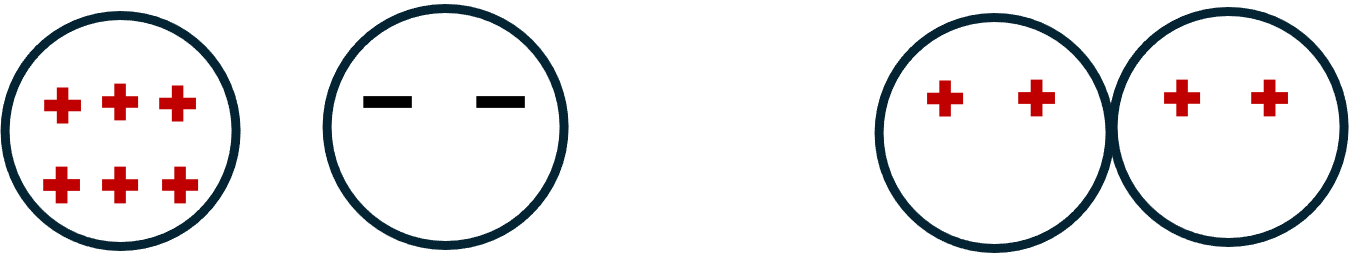
\includegraphics[width=0.8\textwidth]{./pictures/1.png}
        \end{figure}

        原因:\textbf{导体}对电子的束缚力相同,物体之间发生\textbf{电荷转移},带上等量\textbf{同种电荷}  \\    
        物理过程:电中和,电荷量守恒  \\
        (单个导体带电量$\frac{Q_{total}}{n}$,\textbf{正负电荷对}显电中性并未消失)

        \newpage

        \item 静电感应: 带电物体棒靠近其他导体
        \begin{figure}[h]
            \centering
            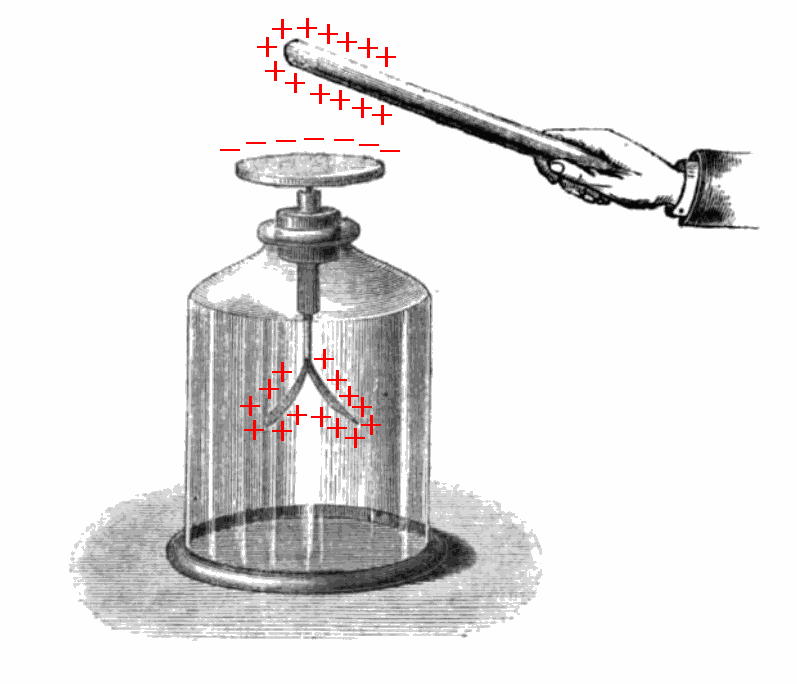
\includegraphics[width=0.25\textwidth]{./pictures/2.png}
        \end{figure}

        原因:导体内的自由电子在库伦力的作用下重新分布 \\
        物理过程:被感导体的内部电荷分布变化,电荷守恒        
    \end{enumerate}


    \section{库伦定律}
    \begin{figure}[h]
        \centering
        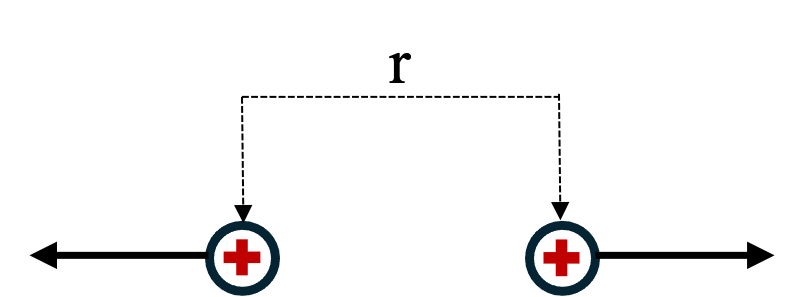
\includegraphics[width=0.45\textwidth]{pictures/3.png}
    \end{figure}
    \begin{thm*}
        库伦定律:\textbf{点电荷}之间存在相互作用力---\textbf{库伦力}
        $$
        F_{c} = k \vdot \frac{Q_{1}Q_{2}}{r^{2}}
        $$
    \end{thm*}
    \begin{itemize}
        \item 经典常量$k = 9 \cross 10^{9} \, N \vdot m^{2} \vdot C^{-2}$
        \item 类比万有引力公式,引力常量$G = 6.67 \cross 10^{-11} \,\, m^{3} \vdot kg^{-1} \vdot s^{-2}$
        \item[] (卡文迪什扭秤实验测量了引力常量)    %\item[]将不会有图标
        $$ 
        F_{G} = G \vdot \frac{mM}{r^{2}} 
        $$
    \end{itemize}
    
    \section{电场与电场强度}
    \begin{enumerate}
        \item 电场: 存在于电荷周围(真实存在却看不见),能\textbf{传递电荷与电荷之间相互作用的物理场}
        \item[] 静电场:观察者相对于电荷静止时所观察到的场 
        \item[] 试探电荷:通过在电荷周围放置一\textbf{电荷}$q_{0}$,观察电荷是否收到力的作用以判断是否存在电场
        \begin{itemize}
            \item[]补充:试探电荷是一假想电荷,且电荷量极小不会对原电场产生影响 
        \end{itemize}
        \item 电场强度:用来表示电场的强弱和方向的物理量
        $$
        F_{c} = (k \vdot \frac{Q}{r^{2}}) \vdot q_{0} = 
        E \vdot q_{0} \quad \llra \quad E = \frac{F_{c}}{q_{0}} \quad (\text{比值定义})
        $$
        符号$E$,单位$ N \vdot C^{-1}$
        \item[] 场源电荷产生的电场强度为: $ E = k \vdot \frac{Q}{r^{2}} $
        \item[] 电场方向:与\textbf{正试探电荷}所受力方向一致
    \end{enumerate}
    




\end{document}